\chapter{Current factorization of the fermion determinant}
\label{chap: FactStd}
The broader goal of this work consists in the exploration of new numerical methods for lattice gauge theories, namely lattice QCD.
\\ As we have already seen, when dynamical fermions are included in lattice gauge theories, we require the Grassmann quark fields to be analytically integrated out first, causing the loss of the manifest locality of the action and of the observables (see Chap. 2.1), as the quark determinant and propagator are non-local functionals of the background gauge fields. 
 Typically, as we have explicitly done for the Schwinger Model, the resulting effective gauge theory is simulated with variants of the hybrid Monte Carlo algorithm. The urge of finding different numerical approaches comes from the fact that the standard Monte Carlo evaluation of most hadronic correlators, with some relevant exceptions (e.g. the pion two-point function), is affected by an exponential degradation of the signal-to-noise ratio (S/N) \cite{PARISI1984203,Lepage:1989hd}. Namely, the variance of a correlator decays exponentially in the time-separation between sink and source with a faster rate than the signal itself.
 \\ Throughout the years many noise-reduction ideas have been developed to tackle down this problem, for instance \textit{multilevel algorithms}, which have been applied to lattice Yang-Mills theories for a long time \cite{L_scher_2001, Meyer_2003, Della_Morte_2009, Della_Morte_2011}, where the local building blocks of the observables are computed independently, so that the degradation of the S/N is avoided.
 \\ Multilevel algorithms in theories with dynamical fermions are more complicated to implement, due to the non-localities mentioned above. To make these techniques feasible, over the last two decades there have been several attempts to rewrite the fermion determinant through a local bosonic field theory. 
 The main ingredients are a factorization of the gauge-field dependence of the quark determinant in lattice QCD with Wilson fermions, based on the domain decomposition of the lattice \cite{L_scher_2004, L_scher_2005, C__2016, C__2017, Giusti_2022}, and the introduction of multi-boson auxiliary fields living on the boundaries of the aforementioned domains \cite{L_scher_1994}. This combination leads to a bosonic action which is local in the block gauge, pseudofermion and multi-boson fields, and together with the factorization of fermionic observables \cite{C__2016} it makes it feasible to conduce multilevel simulations in lattice QCD.
 \\ Many numerical tests have been performed (e.g. \cite{Giusti_2018, Dalla_Brida_2021}), and in this chapter we will review the factorization of the quark determinant presented in \cite{C__2017}. In this work the lattice gets decomposed in overlapping domains along one dimension only, although lately it has been proposed a four-dimensional generalization of this technique \cite{Giusti_2022}. From numerical experience, we can conjecture that contributions which depend on gauge fields living in different regions are suppressed exponentially in the time-separation between sink and source \cite{C__2016}, hence we can control the magnitude of such contributions by tuning the thickness of the overlapping region between the domains of interest.

 \section{Block decomposition of the determinant}

 The goal of this process consists in the decomposition of the effective fermion action in contributions which depend only on the local block gauge, pseudofermion and multiboson fields.
 Consider a non-overlapping 3-block decomposition of the lattice, where each block $\Lambda_i$ $(i = 0, 1, 2)$ may be the union of disconnected regions, but we require that the Dirac operator cannot connect points from $\Lambda_0$ and $\Lambda_2$. Without loss of generality, we can implement periodic and open boundary conditions in the spatial and temporal directions, respectively. Minor adjustements are required to implement periodic boundary conditions in the time direction. Figure \eqref{fig: Decomp} depicts this decomposition in three thick time slices $\Lambda_i$. 
 \begin{figure}
     \centering


\tikzset{every picture/.style={line width=0.75pt}} %set default line width to 0.75pt        

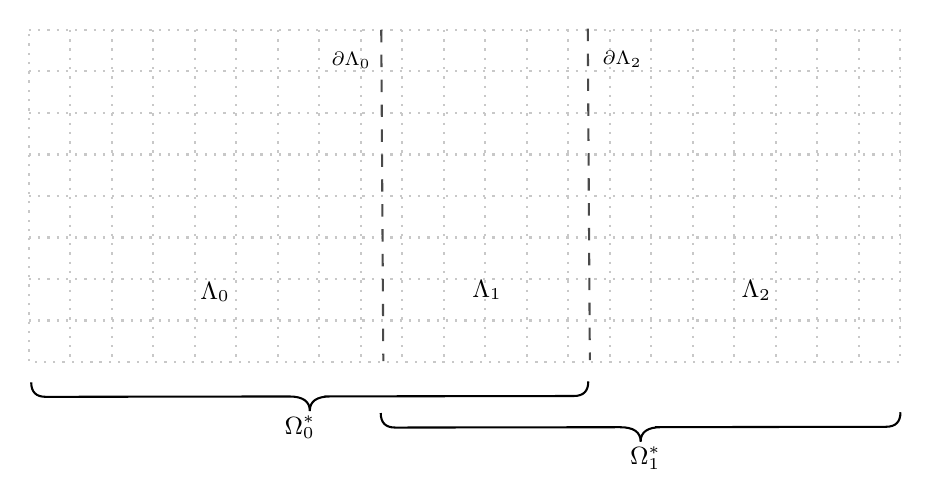
\begin{tikzpicture}[x=0.75pt,y=0.75pt,yscale=-1,xscale=1]
%uncomment if require: \path (0,300); %set diagram left start at 0, and has height of 300

%Shape: Grid [id:dp36732851129859456] 
\draw  [draw opacity=0][dash pattern={on 0.84pt off 2.51pt}] (110.18,50.67) -- (530.18,50.67) -- (530.18,210.67) -- (110.18,210.67) -- cycle ; \draw  [color={rgb, 255:red, 200; green, 200; blue, 200 }  ,draw opacity=1 ][dash pattern={on 0.84pt off 2.51pt}] (130.18,50.67) -- (130.18,210.67)(150.18,50.67) -- (150.18,210.67)(170.18,50.67) -- (170.18,210.67)(190.18,50.67) -- (190.18,210.67)(210.18,50.67) -- (210.18,210.67)(230.18,50.67) -- (230.18,210.67)(250.18,50.67) -- (250.18,210.67)(270.18,50.67) -- (270.18,210.67)(290.18,50.67) -- (290.18,210.67)(310.18,50.67) -- (310.18,210.67)(330.18,50.67) -- (330.18,210.67)(350.18,50.67) -- (350.18,210.67)(370.18,50.67) -- (370.18,210.67)(390.18,50.67) -- (390.18,210.67)(410.18,50.67) -- (410.18,210.67)(430.18,50.67) -- (430.18,210.67)(450.18,50.67) -- (450.18,210.67)(470.18,50.67) -- (470.18,210.67)(490.18,50.67) -- (490.18,210.67)(510.18,50.67) -- (510.18,210.67) ; \draw  [color={rgb, 255:red, 200; green, 200; blue, 200 }  ,draw opacity=1 ][dash pattern={on 0.84pt off 2.51pt}] (110.18,70.67) -- (530.18,70.67)(110.18,90.67) -- (530.18,90.67)(110.18,110.67) -- (530.18,110.67)(110.18,130.67) -- (530.18,130.67)(110.18,150.67) -- (530.18,150.67)(110.18,170.67) -- (530.18,170.67)(110.18,190.67) -- (530.18,190.67) ; \draw  [color={rgb, 255:red, 200; green, 200; blue, 200 }  ,draw opacity=1 ][dash pattern={on 0.84pt off 2.51pt}] (110.18,50.67) -- (530.18,50.67) -- (530.18,210.67) -- (110.18,210.67) -- cycle ;
%Straight Lines [id:da8151691865200523] 
\draw [color={rgb, 255:red, 74; green, 74; blue, 74 }  ,draw opacity=1 ] [dash pattern={on 4.5pt off 4.5pt}]  (280.03,50.61) -- (281.03,210.28) ;
%Straight Lines [id:da2624795881970642] 
\draw [color={rgb, 255:red, 74; green, 74; blue, 74 }  ,draw opacity=1 ] [dash pattern={on 4.5pt off 4.5pt}]  (379.53,50.08) -- (380.53,209.75) ;
%Shape: Brace [id:dp41866974630216447] 
\draw   (111.38,220.45) .. controls (111.39,225.12) and (113.72,227.45) .. (118.39,227.44) -- (235.59,227.26) .. controls (242.26,227.25) and (245.59,229.57) .. (245.6,234.24) .. controls (245.59,229.57) and (248.92,227.24) .. (255.59,227.23)(252.59,227.23) -- (372.79,227.04) .. controls (377.46,227.03) and (379.79,224.7) .. (379.78,220.03) ;
%Shape: Brace [id:dp9584637663157783] 
\draw   (279.78,235.25) .. controls (279.79,239.92) and (282.12,242.25) .. (286.79,242.24) -- (394.99,242.07) .. controls (401.66,242.06) and (404.99,244.39) .. (405,249.06) .. controls (404.99,244.39) and (408.32,242.05) .. (414.99,242.04)(411.99,242.05) -- (523.19,241.87) .. controls (527.86,241.86) and (530.19,239.53) .. (530.18,234.86) ;

% Text Node
\draw (231.99,235.07) node [anchor=north west][inner sep=0.75pt]  [font=\small]  {$\Omega _{0}^{*}$};
% Text Node
\draw (398.39,249.87) node [anchor=north west][inner sep=0.75pt]  [font=\small]  {$\Omega _{1}^{*}$};
% Text Node
\draw (191.43,170.7) node [anchor=north west][inner sep=0.75pt]  [font=\small]  {$\Lambda _{0}$};
% Text Node
\draw (322.43,169.7) node [anchor=north west][inner sep=0.75pt]  [font=\small]  {$\Lambda _{1}$};
% Text Node
\draw (452.18,170.07) node [anchor=north west][inner sep=0.75pt]  [font=\small]  {$\Lambda _{2}$};
% Text Node
\draw (254.63,59.7) node [anchor=north west][inner sep=0.75pt]  [font=\scriptsize]  {$\partial \Lambda _{0}$};
% Text Node
\draw (385.23,59.5) node [anchor=north west][inner sep=0.75pt]  [font=\scriptsize]  {$\partial \Lambda _{2}$};


\end{tikzpicture}

     \caption{Decomposition of the lattice in three thick time slices.}
     \label{fig: Decomp}
 \end{figure}
 \\ Given this domain-decomposition, we can write the hermitian $\mathcal{O}(a)$-improved massive Dirac operator $Q = \gamma_5 D$ (see Appendix \ref{app: Wilson improved op}) in a block form\footnote{For a broader view on the block terminology and decomposition, see Ref. \cite{C__2017}. To keep the
notation compact, a block matrix $Q_{\Lambda_{i,j}}$ denotes either a single block of the whole quark matrix, or the full matrix
with just that block different from zero.}:
 \begin{equation}\label{Q}
    Q = \begin{pmatrix}
 Q_{\Lambda_{0,0}} & Q_{\Lambda_{0,1}} & 0  \\
   Q_{\Lambda_{1,0}} & Q_{\Lambda_{1,1}} & Q_{\Lambda_{1,2}} \\
   0 & Q_{\Lambda_{2,1}} & Q_{\Lambda_{2,2}} \\
\end{pmatrix}
\end{equation}
Since we will refer frequently to quark fields which live in a particular block, it is convenient to define projector operators:
\begin{equation}
    [P_{\Lambda_i}\psi](x) = \left\{ \begin{array}{rcl} \psi(x) \hspace{3mm} \mbox{if} \hspace{2mm} x \in \Lambda_i \\ 0  \hspace{3mm} \mbox{elsewhere}  \\ \end{array} \right.
\end{equation}
which act on subspaces of fermion fields with support in the domain $\Lambda_i$. \\ Analogously, we can define projectors associated with quark fields living on inner and outer boundaries of each domain, namely $P_{\partial \Lambda_i}$ and $P_{\partial \Lambda_i^*}$. We define the inner boundary of a block to be the set of points at a unitary distance from the previous and the following block, and these projectors satisfy the relation:
\begin{equation}
    P_{\partial \Lambda_i} Q_{\Lambda_{i, j}} = Q_{\Lambda_{i, j}} P_{\partial \Lambda_j} = Q_{\Lambda_{i,j}} \hspace{5mm} i \neq j
\end{equation}
Notice that $P_{\Lambda_i}$ labels the corresponding projector independently from the dimensionality of the space where it acts on.
\\ Since we will employ a two-block partitioning of the lattice, let us define the two block operators:
\begin{equation}
    Q_{\Omega_i^*} = \begin{pmatrix}
 Q_{\Lambda_{i,i}} & Q_{\Lambda_{i,i+1}} \\
   Q_{\Lambda_{i+1,i}} & Q_{\Lambda_{i+1,i+1}} \\
\end{pmatrix}
\end{equation}
where $\Omega_i^* = \Lambda_i \cup \Lambda_{i+1}$ and $i = 0, 1$. The factorization of the determinant of $Q$ is realized as follows.
\\ Consider the partitions $\Gamma = \Lambda_0 \cup \Lambda_2$ and $\Gamma^* = \Lambda_1$. Using the Schur decomposition \eqref{Schur} on $Q$ we can write:
\begin{equation}\label{det Q}
    \det Q = \det Q_{\Lambda_{1,1}} \det S_{\Gamma} = \det Q_{\Lambda_{1,1}} \det \begin{pmatrix}
        Q_{\Lambda_{0,0}} - Q_{\Lambda_{0,1}}Q^{-1}_{\Lambda_{1,1}}Q_{\Lambda_{1,0}} & - Q_{\Lambda_{0,1}}Q^{-1}_{\Lambda_{1,1}}Q_{\Lambda_{1,2}} \\
        \\
        - Q_{\Lambda_{2,1}}Q^{-1}_{\Lambda_{1,1}}Q_{\Lambda_{1,0}} & Q_{\Lambda_{2,2}} - Q_{\Lambda_{2,1}}Q^{-1}_{\Lambda_{1,1}}Q_{\Lambda_{1,2}} \\ 
    \end{pmatrix}
\end{equation}
where $S_\Gamma$ is the Schur complement associated with $\Gamma.$ Since the inverse of the Schur complement of a matrix coincides with the matrix inverse if the latter acts upon fields defined in the same block, we can notice that:
\begin{equation}
    \begin{split}
        P_{\Lambda_0} Q^{-1}_{\Omega^*_0} P_{\Lambda_0} = S_{\Omega^*_0}^{-1} = \left[ Q_{\Lambda_{0,0}} - Q_{\Lambda_{0,1}}Q^{-1}_{\Lambda_{1,1}}Q_{\Lambda_{1,0}}  \right]^{-1} \\
        P_{\Lambda_2} Q^{-1}_{\Omega^*_1} P_{\Lambda_2} = S_{\Omega^*_1}^{-1} = \left[ Q_{\Lambda_{2,2}} - Q_{\Lambda_{2,1}}Q^{-1}_{\Lambda_{1,1}}Q_{\Lambda_{1,2}}  \right]^{-1} \\
    \end{split}
\end{equation}
For instance, we can conjecture that if we consider two points $x, y \in \Lambda_0$, then $Q^{-1}(x,y)$ is going to be well approximated by $Q_{\Omega_0^*}^{-1}$, up to corrections suppressed exponentially as $\sim\exp(-M_{\pi} \Delta)$, where $M_\pi$ is the pion mass and $\Delta$ is the thickness of the central block $\Lambda_1$ (see Ref. \cite{C__2016}). Then one can use Eq. \eqref{schur det} on \eqref{det Q} to recast it as:
\begin{equation}
    \det Q = \frac{1}{\det Q_{\Lambda_{1,1}}^{-1} \det \left[ P_{\Lambda_0} Q^{-1}_{\Omega^*_0} P_{\Lambda_0} \right] \det \left[ P_{\Lambda_2} Q^{-1}_{\Omega^*_1} P_{\Lambda_2}  \right] } \det \begin{pmatrix}
        1 & P_{\Lambda_0 Q_{\Omega^*_{0}}^{-1} Q_{\Lambda_{1,2}}} \\ 
        P_{\Lambda_2} Q_{\Omega_1^*}^{-1} Q_{\Lambda_{1,0}} & 1 \\
    \end{pmatrix}
\end{equation}
Finally, using again Eq. \eqref{Schur}, we can rewrite the last determinant of the previous expression as the determinant of a matrix acting on one of the boundaries only:
\begin{equation}\label{final det}
    \det \begin{pmatrix}
        1 & P_{\Lambda_0 Q_{\Omega^*_{0}}^{-1} Q_{\Lambda_{1,2}}} \\ 
        P_{\Lambda_2} Q_{\Omega_1^*}^{-1} Q_{\Lambda_{1,0}} & 1 \\
    \end{pmatrix} = \det \left(1 - P_{\partial \Lambda_0} Q_{\Omega_0^*}^{-1} Q_{\Lambda_{1,2}} P_{\partial \Lambda_2} Q_{\Omega_1^{*}}^{-1} Q_{\Lambda_{1,0}} P_{\partial \Lambda_0} \right)
\end{equation}
If we call:
\begin{equation}\label{w}
  w =  P_{\partial \Lambda_0} Q_{\Omega_0^*}^{-1} Q_{\Lambda_{1,2}} P_{\partial \Lambda_2} Q_{\Omega_1^{*}}^{-1} Q_{\Lambda_{1,0}} P_{\partial \Lambda_0}
\end{equation}
we can write the factorized formula for the Dirac-Wilson operator determinant:
\begin{equation}\label{det Q}
    \det Q = \frac{1}{\det Q_{\Lambda_{1,1}}^{-1} \det \left[ P_{\Lambda_0} Q^{-1}_{\Omega^*_0} P_{\Lambda_0} \right] \det \left[ P_{\Lambda_2} Q^{-1}_{\Omega^*_1} P_{\Lambda_2}  \right] } \det (1 - w)
\end{equation}
Indeed we have that:
\begin{itemize}
    \item $\det Q_{\Lambda_{1,1}}^{-1}$ depends only on the gauge fields in $\Lambda_1$;
    \item $\left[ P_{\Lambda_0} Q^{-1}_{\Omega^*_0} P_{\Lambda_0} \right]$ depends only on the gauge fields in $\Lambda_0 \cup \Lambda_1$;
    \item $\left[ P_{\Lambda_2} Q^{-1}_{\Omega^*_1} P_{\Lambda_2}  \right]$ depends only on the gauge fields in $\Lambda_1 \cup \Lambda_2$;
    \item $\det (1 - w)$ is a small correction, and it is a function of links defined across the whole lattice. Notice that this determinant is real, since all the other terms in \eqref{det Q} are.
\end{itemize}
Now we should shed more light on the magnitude of $\det(1 - w)$, in order to verify the goodness of this factorization.

\subsection{Magnitude of $w$}
In order to better understand the contribution brought by $w$, it is convenient to recast this matrix in terms of the full propagator $Q^{-1}$.
If we consider two different partitions of the lattice, namely $\Lambda_0 \cup \Lambda_1 + \Lambda_2$ and $\Lambda_0 + \Lambda_1 \cup \Lambda_2$, it is possible to show that:
\begin{equation}\label{boundary prop}
    \begin{split}
        P_{\Lambda_0} Q^{-1}_{\Omega^*_0} Q_{\Lambda_{1,2}} = P_{\partial \Lambda_0} Q^{-1} \{Q_{\Lambda_{1,2}} + Q_{\Lambda_{2,1}} Q_{\Omega_0^*}^{-1} Q_{\Lambda_{1,2}} \} \\ 
         P_{\Lambda_2} Q^{-1}_{\Omega^*_1} Q_{\Lambda_{1,0}} = P_{\partial \Lambda_2} Q^{-1} \{Q_{\Lambda_{1,0}} + Q_{\Lambda_{0,1}} Q_{\Omega_1^*}^{-1} Q_{\Lambda_{1,0}}\}
    \end{split}
\end{equation}
hence in the definition of $w$ we have two propagators between the boundaries of the blocks $\Lambda_0$ and $\Lambda_2$, each one multiplied by an effective boundary operator. A visual representation of $w$ is given in Figure \eqref{fig: op w}.
\begin{figure}
    \centering


\tikzset{every picture/.style={line width=0.75pt}} %set default line width to 0.75pt        

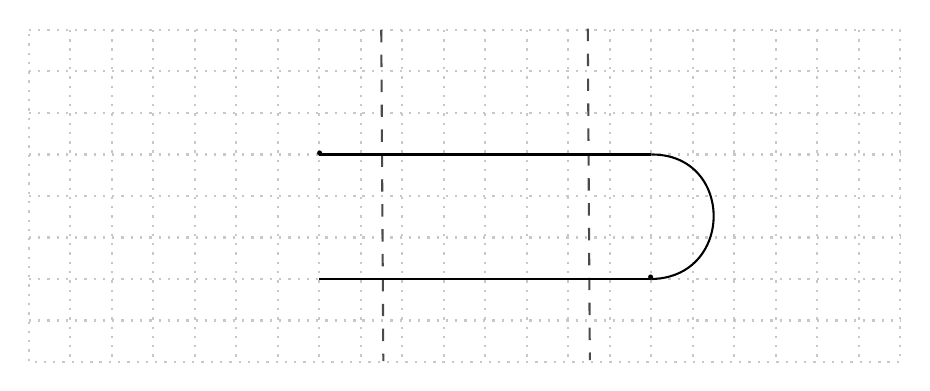
\begin{tikzpicture}[x=0.75pt,y=0.75pt,yscale=-1,xscale=1]
%uncomment if require: \path (0,300); %set diagram left start at 0, and has height of 300

%Shape: Grid [id:dp36732851129859456] 
\draw  [draw opacity=0][dash pattern={on 0.84pt off 2.51pt}] (110.18,50.67) -- (530.18,50.67) -- (530.18,210.67) -- (110.18,210.67) -- cycle ; \draw  [color={rgb, 255:red, 200; green, 200; blue, 200 }  ,draw opacity=1 ][dash pattern={on 0.84pt off 2.51pt}] (130.18,50.67) -- (130.18,210.67)(150.18,50.67) -- (150.18,210.67)(170.18,50.67) -- (170.18,210.67)(190.18,50.67) -- (190.18,210.67)(210.18,50.67) -- (210.18,210.67)(230.18,50.67) -- (230.18,210.67)(250.18,50.67) -- (250.18,210.67)(270.18,50.67) -- (270.18,210.67)(290.18,50.67) -- (290.18,210.67)(310.18,50.67) -- (310.18,210.67)(330.18,50.67) -- (330.18,210.67)(350.18,50.67) -- (350.18,210.67)(370.18,50.67) -- (370.18,210.67)(390.18,50.67) -- (390.18,210.67)(410.18,50.67) -- (410.18,210.67)(430.18,50.67) -- (430.18,210.67)(450.18,50.67) -- (450.18,210.67)(470.18,50.67) -- (470.18,210.67)(490.18,50.67) -- (490.18,210.67)(510.18,50.67) -- (510.18,210.67) ; \draw  [color={rgb, 255:red, 200; green, 200; blue, 200 }  ,draw opacity=1 ][dash pattern={on 0.84pt off 2.51pt}] (110.18,70.67) -- (530.18,70.67)(110.18,90.67) -- (530.18,90.67)(110.18,110.67) -- (530.18,110.67)(110.18,130.67) -- (530.18,130.67)(110.18,150.67) -- (530.18,150.67)(110.18,170.67) -- (530.18,170.67)(110.18,190.67) -- (530.18,190.67) ; \draw  [color={rgb, 255:red, 200; green, 200; blue, 200 }  ,draw opacity=1 ][dash pattern={on 0.84pt off 2.51pt}] (110.18,50.67) -- (530.18,50.67) -- (530.18,210.67) -- (110.18,210.67) -- cycle ;
%Straight Lines [id:da8151691865200523] 
\draw [color={rgb, 255:red, 74; green, 74; blue, 74 }  ,draw opacity=1 ] [dash pattern={on 4.5pt off 4.5pt}]  (280.03,50.61) -- (281.03,210.28) ;
%Straight Lines [id:da2624795881970642] 
\draw [color={rgb, 255:red, 74; green, 74; blue, 74 }  ,draw opacity=1 ] [dash pattern={on 4.5pt off 4.5pt}]  (379.53,50.08) -- (380.53,209.75) ;
%Straight Lines [id:da6638407323679787] 
\draw    (250.18,170.67) -- (410.18,170.67) ;
%Curve Lines [id:da08584860303537212] 
\draw    (410.18,110.67) .. controls (433.55,110.54) and (443.27,130.84) .. (439.33,147.86) .. controls (436.52,159.97) and (426.81,170.41) .. (410.18,170.67) ;
%Straight Lines [id:da2105866998964242] 
\draw    (250.18,110.67) -- (410.18,110.67) ;

% Text Node
\draw (405.2,163.92) node [anchor=north west][inner sep=0.75pt]  [font=\LARGE,rotate=-359.89]  {$\cdot $};
% Text Node
\draw (245.8,104.42) node [anchor=north west][inner sep=0.75pt]  [font=\LARGE,rotate=-359.89]  {$\cdot $};


\end{tikzpicture}

    \caption{Representation of the operator $w$, which acts on a single boundary and can be written as the composition of two propagators between $\partial\Lambda_0$ and $\partial \Lambda_2$. The black lines are full propagators, while the thick dots are insertions of the effective hops; see Eq. \eqref{boundary prop}.}
    \label{fig: op w}
\end{figure}
\\ We conjecture from numerical experience (see Ref. \cite{C__2016}), that if the thickness of the central block $\Delta$ is large enough, each of these propagators will decay exponentially as $\sim \exp(-\frac{1}{2} M_\pi \Delta)$, hence the norm of $w$ will be suppressed $\sim \exp(-M_\pi \Delta)$.

\subsection{Spectrum of $w$}
In order to pair the domain decomposition with the multiboson approach, we need to know more in depth the spectrum of $(1 - w)$.
\\ Given the definition of $w$ in Eq. \eqref{w} and the relation in \eqref{matrix inverse}, we can rewrite $w$ as the product of two Hermitian matrices acting upon $\partial \Lambda_0$, i.e. the inner boundary of $\Lambda_0$:
\begin{equation}
    w = \left[P_{\partial\Lambda_0} Q^{-1}_{\Omega^*_0} P_{\partial\Lambda_0}\right] \cdot \left[ Q_{\Lambda_{0,1}} Q_{\Lambda_{1,1}}^{-1} Q_{\Lambda_{1,2}} Q^{-1}_{\Omega^*_1} Q_{\Lambda_{2,1}} Q_{\Lambda_{1,1}}^{-1} Q_{\Lambda_{1,0}} \right]
\end{equation}
and this allows us to conclude that $w$ is similar to $w^{\dagger}$ (see Ref. \cite{10.2307/2042048}). This in turn implies that the characteristic polynomial of $w$ has real coefficients, and its complex eigenvalues $\delta_i$ come in conjugate pairs. This results in a symmetric spectrum with respect to the real axis, hence the determinant of $(1 - w)$ is real. Since the norm of $w$ is suppressed as $\sim \exp(-M_\pi \Delta)$, we expect the modulus of the eigenvalues $\abs{\delta_i}$ to have the same behaviour.
\\ This leads us to the conclusion that, for a suitably chosen value of $\Delta$, all the eigenvalues of $w$ satisfy $\abs{\delta_i} \ll 1$, resulting in a large spectral gap for $(1 - w)$.
 Consequently, we can express $\det(1-w)$ through an adequate polynomial approximation of $(1 - w)^{-1}.$

 \section{Multiboson factorization}
 The main result of the previous section was the factorization of the quark determinant into terms which depend only on gauge fields in the neighboring thick time slices, resulting from a non-overlapping domain decomposition. The factorization is not complete, as the term $\det(1-w)$ still depends on the link variables defined across the whole lattice, but with a suitable fine tuning of the central block thickness $\Delta$, we can treat this term as a small contribution and express it through a polynomial approximation.
 \subsection{Polynomial approximation}
 Lüscher's original multiboson idea \cite{L_scher_1994} can be generalized to complex matrices \cite{Bori_i_1995, Bori_i_1996, Jegerlehner_1996}, hence the first step we need to take into account is the approximation of the function $1/z$ (with $z \in \mathbb{C}$) via the polynomial:
 \begin{equation}\label{pol}
    P_N (z) \equiv \frac{1 - R_{N+1}(z)}{z} = c_N \prod_{k = 1}^N (z - z_k)
 \end{equation}
 where $N$ is chosen to be even, and the $N$ roots of $P_N(z)$ are obtained by requiring that for the remainder, which is defined in \eqref{remainder}, $R_{N+1}(0) = 1$. The roots $z_k$ of $P_N(z)$ can be chosen to lie on an ellipse passing through the origin of the complex plane with center $1$ and foci $1 \pm c$, hence from \eqref{roots}:
 \begin{equation}
     u_k = 1 - z_k = \cos(\frac{2\pi k}{N+1}) + i \sqrt{1 - c^2} \sin(\frac{2 \pi k}{N + 1}) \hspace{5mm} k = 1, \dots, N
 \end{equation}

 \subsection{Approximation of the determinant}
 We can use the polynomial approximation in \eqref{pol} to express the determinant of $(1 - w)$ as:
 \begin{equation} \label{det approximation}
     \det (1 - w) \det (P_N(1 - w)) = \det (1 - R_{N+1} (1 - w))
 \end{equation}
 therefore, if all the eigenvalues of $w$ satisfy $\abs{\delta_i} \ll 1$, the RHS converges exponentially to 1 as we increase the degree of the polynomial approximation $N$. Given the symmetric structure of the spectrum of $(1 - w)$ with respect to the real axis, we can recast the approximate determinant in a manifestly positive form:
 \begin{equation} \label{approx det}
     \det \left( P_N(1 - w) \right)^{-1} = c \prod_{k = 1}^{N/2} \det^{-1} \big\{ (u_k - w)^{\dagger} (u_k - w) \big\} = c \prod_{k = 1}^{N/2} \det^{-1} \left( W^\dagger_{\sqrt{u_k}} W_{\sqrt{u_k}} \right)
 \end{equation}
 where $c$ is an irrelevant constant, and $W_z$ is defined as:
 \begin{equation}
     W_z = \begin{pmatrix}
         z P_{\partial \Lambda_0} & P_{\partial \Lambda_0 Q_{\Omega_0^*}^{-1} Q_{\Lambda_{1,2}}} \\ 
         P_{\partial \Lambda_2 Q_{\Omega_1^*}^{-1} Q_{\Lambda_{1,0}}} & z P_{\partial \Lambda_2}
     \end{pmatrix}
 \end{equation}
 Notice that in the last equality of \eqref{approx det} we made use of the reverse substitution of the one used in \eqref{final det}.
Indeed the expression with $W_z$ acting on the inner boundaries $\partial \Lambda_0$ and $\partial \Lambda_2$ allows for a fully factorized domain decomposition of the fermion action.
\newpage
\subsection{Multiboson action}
For a system with two quark flavors, we can represent the determinants through scalar fields $\phi_i$ \cite{Weingarten:1980hx} with support in a corresponding domain $\Lambda_i$ ($i = 0, 1, 2$) and $N$ multiboson auxiliary fields $\chi_k$ which live on the outer boundaries of $\Lambda_1$, namely:
\begin{equation}
    \begin{split}
        \frac{\det Q^2}{\det \{ 1 - R_{N+1}(1 - w) \}^2} = \frac{1}{\det \left[Q_{\Lambda_{1,1}}^{-1}\right]^2 \det \left[ P_{\Lambda_0} Q^{-1}_{\Omega^*_0} P_{\Lambda_0} \right]^2 \det \left[ P_{\Lambda_2} Q^{-1}_{\Omega^*_1} P_{\Lambda_2}  \right]^2} \cross \\
        \cross \det \{ P_N(1 - w) \}^{-2} = c' \cdot \int \left[d\phi_0 d\phi_0^\dagger \right] e^{-\abs{P_{\Lambda_0} Q_{\Omega_0^*}^{-1} \phi_0}^2} \cdot \int \left[d\phi_1 d\phi_1^\dagger \right] e^{-\abs{ Q_{\Lambda_{1,1}}^{-1} \phi_0}^2} \cdot \\
        \cdot \int \left[d\phi_2 d\phi_2^\dagger \right] e^{-\abs{P_{\Lambda_2} Q_{\Omega_1^*}^{-1} \phi_2}^2} \cdot \prod_{k = 1}^{N} \bigg\{  \int \left[d\chi_l d\chi_k^\dagger \right] e^{-\abs{ W_{\sqrt{u_k}} \chi_k }^2} \bigg\}
    \end{split}
\end{equation}
where $c'$ is another irrelevant numerical constant.
\\ Since the auxiliary fields $\chi_k$ live on the outer boundaries of $\Lambda_1$, they can be decomposed as $\chi_k = \eta_k + \xi_k$, where $\eta_k = P_{\partial\Lambda_0} \chi_k$ and $\xi_k = P_{\partial \Lambda_2} \chi_k$. This allows us to split explicitly the contributions from the different inner boundaries $\partial \Lambda_0$ and $\partial \Lambda_2$ as:
\begin{equation}
\begin{split}
     \abs{W_z \chi_k}^2 = & \abs{z}^2 \abs{\eta_k}^2 + \abs{z}^2 \abs{\xi_k}^2 + \abs{P_{\partial \Lambda_2} Q_{\Omega_1^*}^{-1} Q_{\Lambda_{1,0}} \eta_k }^2 + \\ & + \abs{P_{\partial \Lambda_0} Q_{\Omega_0^*}^{-1} Q_{\Lambda_{1,2}} \xi_k }^2 + \left[ z\left( \xi_k, Q_{\Lambda_{2,1}} Q_{\Omega_0^*}^{-1} \eta_k \right) + z^* \left(\xi_k, Q_{\Omega_1^*}^{-1} Q_{\Lambda_{1,0}} \eta_k \right) + c.c. \right]
\end{split}
\end{equation}
and the dependence of the bosonic action from the gauge fields in block $\Lambda_0$ and $\Lambda_2$ is thus factorized. Notice that the terms in the last expression which will contribute to the forces in the block $\Lambda_0$ always start (or end) on the inner boundary of $\Lambda_2$ and viceversa.
\\ These terms contain one boundary to boundary quark propagator, which is suppressed exponentially in $\Delta$ accordingly to what we have seen before (see \eqref{boundary prop}), and so will be the corresponding forces.

\subsection{Order of the polynomial}
By making use of the definitions in Appendix \ref{app:approx}, we can fix the order of the polynomial accordingly to the desired precision. This guarantees that:
\begin{equation}
    \max_{\norm{v} = 1} \norm{\left[ 1 - (1-w)P_N(1-w) \right] v} \leq \max_i \abs{\delta_i}^{N+1} = \abs{\delta}_{\textrm{max}}^{N+1}
\end{equation}
where $v$ is a generic vector on which $w$ acts. From Eq. \eqref{det approximation} we can formalize that, when $\abs{\delta}_{\textrm{max}}^{N+1} \ll 1$ and $\Tr R_{N+1}(1-w) \ll 1$:
\begin{equation}
    \det(1-w) \det P_N(1-w) = 1 - \Tr R_{N+1}(1 - w) + \dots
\end{equation}
Then if one stops at the first order in the expansion, the relative error on the determinant approximation is given by:
\begin{equation}
    \abs{\Tr R_{N+1}(1 - w)} \leq \sum_{i} \abs{\delta_i}^{N+1} \leq \sum_{i = 1}^{N_{ev}} \abs{\delta_i}^{N+1} + (6L^3 - N_{ev}) \abs{\delta_{N_{ev} +1}}^{N+1}
\end{equation}
where in the last inequality the contribution from the $N_{ev}$ eigenvalues with the highest modules, i.e. $\abs{\delta_i}$ sorted decreasingly, has been treated separately and $L$ is the spatial extension in lattice units. The term on the RHS of the last expression will not be cospicuous if most of the eigenvalues have a modulus significantly smaller than $\abs{\delta_i}$ and the degree of the polynomial $N$ is large.
Given the distribution of the eigenvalues of $w$, different choices can be made for the polynomial approximating $(1-w)^{-1}$, including a circle centered in $1$ and with radius $1$ (see Appendix \ref{app:approx}) or an ellipse where the parameter $c$ is adequately tuned.

\subsection{Reweighting factor}
Once that we factorized the determinant and introduced multiboson fields, a given correlation function of a string of fields $O$ can be written as:
\begin{equation}
    \langle O \rangle = \frac{\langle O \mathcal{W}_N \rangle_N}{\langle \mathcal{W} \rangle_N } = \frac{\langle O_{\textrm{fact}\rangle}}{\langle \mathcal{W}_N \rangle_N} + \frac{\langle O\mathcal{W}_N - O_{\textrm{fact}} \rangle_N}{\langle \mathcal{W}_N \rangle_N}
\end{equation}
where $O_{\textrm{fact}}$ is a precise factorized approximation of $O$ (see \cite{C__2016} for some examples), $\mathcal{W}_N$ is a reweighting factor and $\langle \cdot \rangle_N$ represents an expectation value taken in a theory with $N$ multiboson fields. The factorization of the observables alongside the introduction of the multiboson action allow us to perform a multi-level simulation scheme for the computation of $\langle O_{\textrm{fact}} \rangle_N$, where the gauge configurations are drawn accordingly to the multiboson action with finite $N$. All the other quantities in the previous expression can be computed with a one-level Monte Carlo algorithm. In the case of two quark flavors, the reweighting factor $\mathcal{W}_N$ assumes the expression:
\begin{equation}
    \mathcal{W_N} = \det{1 - R_{N+1}(1-w)}^2
\end{equation}
and if the roots of the polynomial approximation are chosen to lie on a circle rather than on an ellipse (see Appendix \eqref{app:approx}), a simplification occurs and we can use $R_{N+1}(1-w) = w^{N+1}$.